\chapter{Results and Discussion}
In order to verify the proposed method we test our method with two datasets. First we apply our method to the data collected from the test bed which is described in the chapter \ref{chp:testbed} . Next we make use of the data released by the WSU smart home project\footnote{http://ailab.wsu.edu/casas/datasets/} \cite{cook2009assessing}.
\section{HTC34 testbed}
As described earlier the testbed consists of a 8 sensors arranged in a $4 \times 2$ grid. The sensor has a filed of view of radius 2.6m the calculation is explained in appendix \ref{app:fov}. The overlap between the field of view of sensors placed on the grid is as shown in the figure \ref{fig:fov} With the help of the co-ordinates of the sensors we obtain the adjacency matrix of the grid as shown in the figure \ref{fig:gamGraph}.
%\subsection{Determination of Window length}
%The first step in evaluation of our method is to obtain the energy stream from the raw data. To obtain the energy stream we use a moving window with 50\% overlap. We determine this window length empirically. As we already know the neighbors of every sensor
%We determine the window length empirically. We calculate 



\begin{figure}
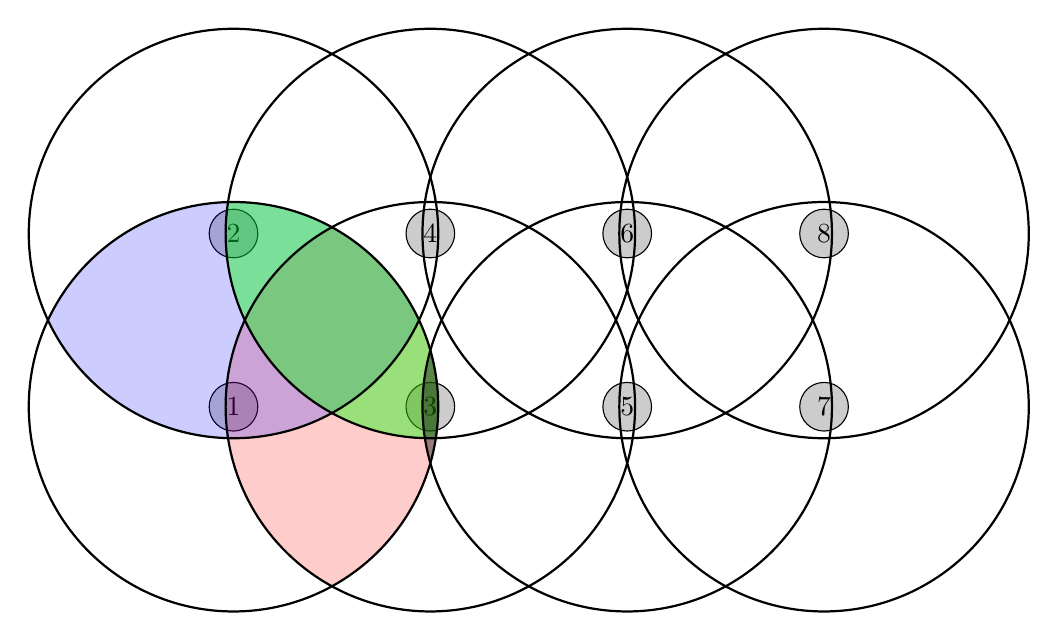
\begin{tikzpicture}
\node[circle,draw=black,fill=white!80!black,minimum size=5] (1) at (0,0)     {1} ;
\node[circle,draw=black,fill=white!80!black,minimum size=5] (3) at (2.5,0)   {3};
\node[circle,draw=black,fill=white!80!black,minimum size=5] (5) at (5,0)     {5};
\node[circle,draw=black,fill=white!80!black,minimum size=5] (7) at (7.5,0)   {7};
\node[circle,draw=black,fill=white!80!black,minimum size=5] (2) at (0,2.2)   {2};
\node[circle,draw=black,fill=white!80!black,minimum size=5] (4) at (2.5,2.2) {4};
\node[circle,draw=black,fill=white!80!black,minimum size=5] (6) at (5,2.2)   {6};
\node[circle,draw=black,fill=white!80!black,minimum size=5] (8) at (7.5,2.2) {8};

\begin{scope}
  \clip (0,0)      circle(2.6);
  \fill[red,fill opacity=.2] (2.5,0)    circle(2.6);
\end{scope}
\begin{scope}
  \clip (0,0)      circle(2.6);
  \fill[blue,fill opacity=.2] (0,2.2)    circle(2.6);
\end{scope}
\begin{scope}
  \clip (0,0)      circle(2.6);
  \fill[green,fill opacity=.4] (2.5,2.2)    circle(2.6);
\end{scope}
\begin{scope}
  \clip (0,0)      circle(2.6);
  \fill[black,fill opacity=.4] (5,0)    circle(2.6);
\end{scope}

\draw[thick](0,0)      circle(2.6);
\draw[thick](2.5,0)    circle(2.6);
\draw[thick](5,0)      circle(2.6);
\draw[thick](7.5,0)    circle(2.6);
\draw[thick](0,2.2)    circle(2.6);
\draw[thick](2.5,2.2)  circle(2.6);
\draw[thick](5,2.2)    circle(2.6);
\draw[thick](7.5,2.2)  circle(2.6);

\end{tikzpicture}
\centering
\caption{Overlapping field of view of the sensors on the vertex with the overlapping field of view for sensor 1 highlighted in color}
\label{fig:fov}
\end{figure}



\begin{figure}
\includegraphics[scale=0.5]{./pics/adjacency.png}
\caption{Grid adjacency matrix for the grid and its corresponding adjacency graph}
\label{fig:gamGraph}


\end{figure}

%\section{Convergence Time}
%An important aspect to know in an data driven method is to know how much of data is required in order to get accurate results. For this purpose we 
\section{Results}
The Grid adjacency matrix for the grid and corresponding grid graph is as shown in figure \ref{fig:gamGraph}. The computed correlation values for one of the dataset  is as shown in the figure \ref{fig:corrMatrix}.
We evaluate the performance with 10 different datasets. We were able to map the sensors onto the grid accurately upto rotational symmetry using the weighted grid adjacency matrix and calculating the $GCS$. The mappings obtained are as shown in the figure \ref{fig:arrangement}.
Table \ref{tab:resHTC} provides details about the number of states visited, number of mappings between the MST and the grid, and the number of mappings obtained as the solution from the developed method and the percentage error. As can be seen from table we obtain 0\% error for all the datasets. 
The number of states visited(includes all the intermediate states) and the number of mappings is lesser than number of possible arrangements which is $8! = 40320$. Number of mappings is almost 14 times lesser than brute force method.

\begin{figure}
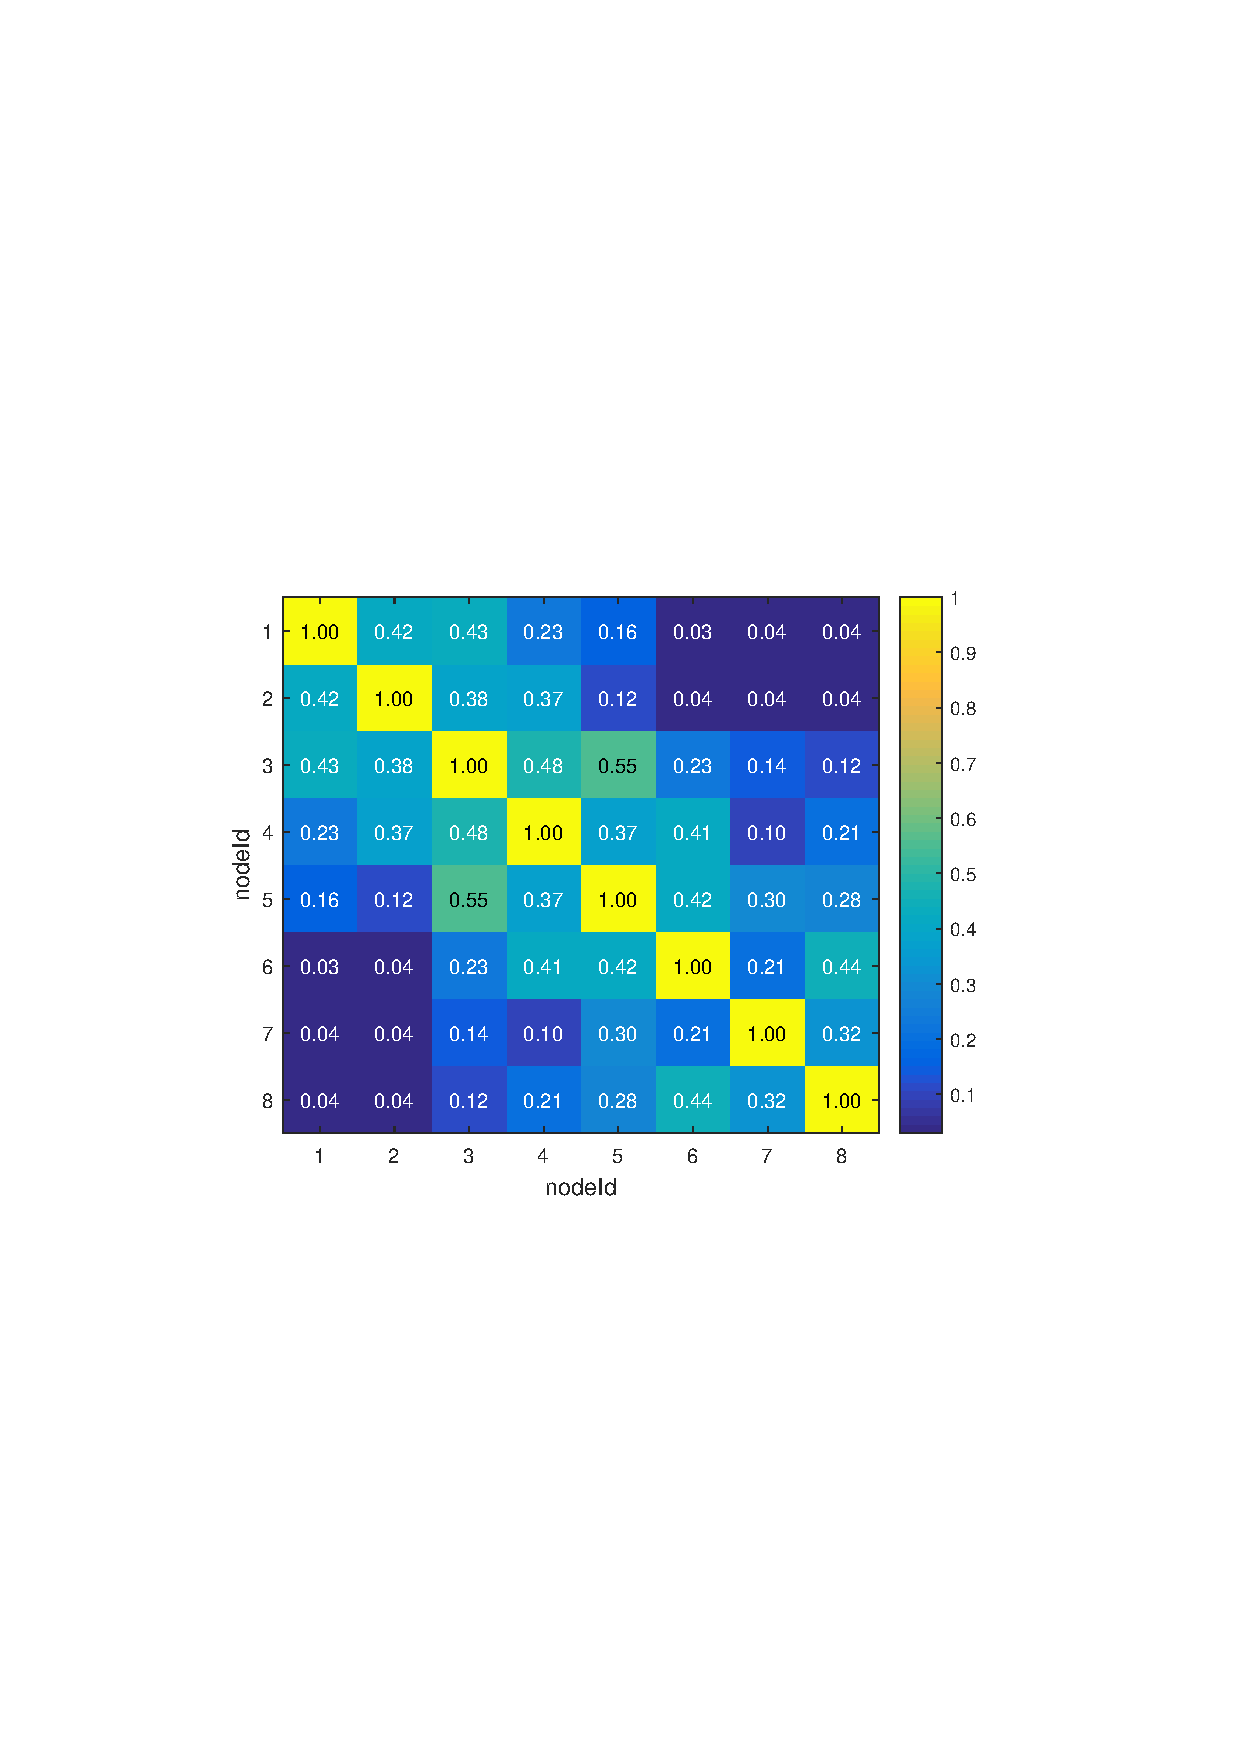
\includegraphics[scale=0.75]{./pics/correlation.pdf}
\caption{Correlation matrix R}
\centering
\label{fig:corrMatrix}

\end{figure}

\begin{table}[]
\centering
\caption{Results obtained from the HTC34 testbed.}
\label{tab:resHTC}
\begin{tabular}{|c|c|c|c|c|}
\hline
dataset & \begin{tabular}[c]{@{}c@{}}Number of \\ states visited\end{tabular} & Mappings & \begin{tabular}[c]{@{}c@{}}Solution\\ Mapping\end{tabular} & Error \\ \hline
1       & 11888                                                               & 2744     & 4                                                          & 0     \\ \hline
2       & 12360                                                               & 2744     & 4                                                          & 0     \\ \hline
3       & 12144                                                               & 2664     & 4                                                          & 0     \\ \hline
4       & 11984                                                               & 2752     & 4                                                          & 0     \\ \hline
5       & 11736                                                               & 2592     & 4                                                          & 0     \\ \hline
6       & 11888                                                               & 2744     & 4                                                          & 0     \\ \hline
7       & 11776                                                               & 2736     & 4                                                          & 0     \\ \hline
8       & 11368                                                               & 2664     & 4                                                          & 0     \\ \hline
9       & 11752                                                               & 2656     & 4                                                          & 0     \\ \hline
10      & 11368                                                               & 2664     & 4                                                          & 0     \\ \hline
11      & 11368                                                               & 2664     & 4                                                          & 0     \\ \hline
\end{tabular}
\end{table}

\begin{figure}
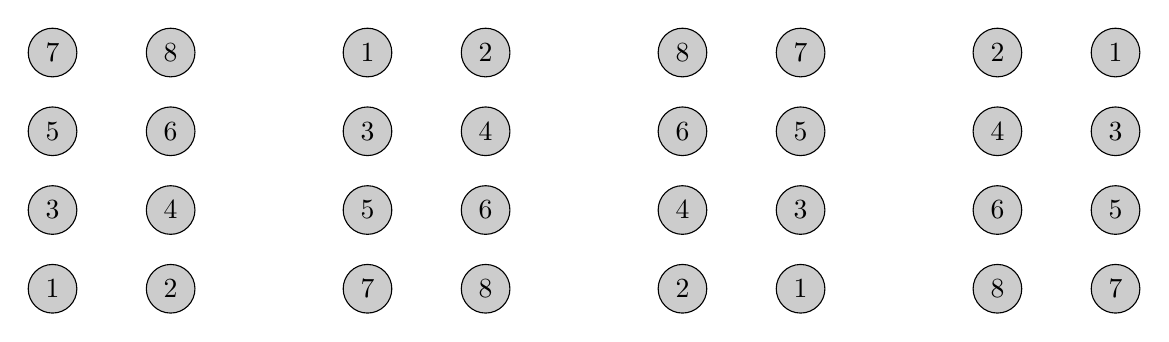
\begin{tikzpicture}
\begin{scope}
\node[circle,draw=black,fill=white!80!black,minimum size=3] (1) at (0,0)   {1};
\node[circle,draw=black,fill=white!80!black,minimum size=3] (2) at (1.5,0) {2};
\node[circle,draw=black,fill=white!80!black,minimum size=3] (3) at (0,1)   {3};
\node[circle,draw=black,fill=white!80!black,minimum size=3] (4) at (1.5,1) {4};
\node[circle,draw=black,fill=white!80!black,minimum size=3] (5) at (0,2)   {5};
\node[circle,draw=black,fill=white!80!black,minimum size=3] (6) at (1.5,2) {6};
\node[circle,draw=black,fill=white!80!black,minimum size=3] (7) at (0,3)   {7};
\node[circle,draw=black,fill=white!80!black,minimum size=3] (8) at (1.5,3) {8};
\end{scope}
\begin{scope}[shift={(4,0)}]
\node[circle,draw=black,fill=white!80!black,minimum size=3] (1) at (0,0)   {7};
\node[circle,draw=black,fill=white!80!black,minimum size=3] (2) at (1.5,0) {8};
\node[circle,draw=black,fill=white!80!black,minimum size=3] (3) at (0,1)   {5};
\node[circle,draw=black,fill=white!80!black,minimum size=3] (4) at (1.5,1) {6};
\node[circle,draw=black,fill=white!80!black,minimum size=3] (5) at (0,2)   {3};
\node[circle,draw=black,fill=white!80!black,minimum size=3] (6) at (1.5,2) {4};
\node[circle,draw=black,fill=white!80!black,minimum size=3] (7) at (0,3)   {1};
\node[circle,draw=black,fill=white!80!black,minimum size=3] (8) at (1.5,3) {2};
\end{scope}
\begin{scope}[shift={(8,0)}]
\node[circle,draw=black,fill=white!80!black,minimum size=3] (1) at (0,0)   {2};
\node[circle,draw=black,fill=white!80!black,minimum size=3] (2) at (1.5,0) {1};
\node[circle,draw=black,fill=white!80!black,minimum size=3] (3) at (0,1)   {4};
\node[circle,draw=black,fill=white!80!black,minimum size=3] (4) at (1.5,1) {3};
\node[circle,draw=black,fill=white!80!black,minimum size=3] (5) at (0,2)   {6};
\node[circle,draw=black,fill=white!80!black,minimum size=3] (6) at (1.5,2) {5};
\node[circle,draw=black,fill=white!80!black,minimum size=3] (7) at (0,3)   {8};
\node[circle,draw=black,fill=white!80!black,minimum size=3] (8) at (1.5,3) {7};
\end{scope}
\begin{scope}[shift={(12,0)}]
\node[circle,draw=black,fill=white!80!black,minimum size=3] (1) at (0,0)   {8};
\node[circle,draw=black,fill=white!80!black,minimum size=3] (2) at (1.5,0) {7};
\node[circle,draw=black,fill=white!80!black,minimum size=3] (3) at (0,1)   {6};
\node[circle,draw=black,fill=white!80!black,minimum size=3] (4) at (1.5,1) {5};
\node[circle,draw=black,fill=white!80!black,minimum size=3] (5) at (0,2)   {4};
\node[circle,draw=black,fill=white!80!black,minimum size=3] (6) at (1.5,2) {3};
\node[circle,draw=black,fill=white!80!black,minimum size=3] (7) at (0,3)   {2};
\node[circle,draw=black,fill=white!80!black,minimum size=3] (8) at (1.5,3) {1};
\end{scope}
\end{tikzpicture}
\caption{Arrangements obtained as solution for the HTC34 testbed}
\label{fig:arrangement}
\centering
\end{figure}

\section{WSU Tokyo testbed}
We evaluate our method using the WSU smart workplace testbed\cite{cook2010detection}, a publicly available data set. The testbed is located in a 12.2m $\times$ 10.9m  lab,  where students performed their normal work routine. The data was collected over a period of 4 months. 
The testbed consists of 43 motion sensors, placed as shown in the figure \ref{fig:casas}. The sensors field of view is $1.2m \times 1.2m$. In appendix \ref{app:wsuGrid} we provide a detailed explanation about how we obtain the grid adjacency matrix for the testbed.
First we choose a $4 \times 3$ grid which includes sensors 27, 22, 15, 28, 23, 16, 29, 24, 17, 30, 25, 18. This grid was chosen as it is mentioned in \cite{cook2010detection} that the region covered by these sensors is more active.
The data from the WSU testbed is represented in the form of a four tuple as shown in table \ref{tab:WSUDATA}. We re-sample the data at 100ms.

\begin{table}[]
\centering
\caption{Data structure of the WSU data.}
\label{tab:WSUDATA}
\begin{tabular}{|c|c|c|c|}
\hline
Date       & Time            & sensor & state \\ \hline
2008-01-02 & 08:02:19.58542  & M39    & ON    \\ \hline
2008-01-02 & 08:02:19.884461 & M41    & OFF   \\ \hline
2008-01-02 & 08:02:20.297468 & M32    & ON    \\ \hline
2008-01-02 & 08:02:20.297468 & M32    & ON    \\ \hline
2008-01-02 & 08:02:20.689425 & M31    & ON    \\ \hline
2008-01-02 & 08:02:21.957307 & M44    & OFF   \\ \hline
2008-01-02 & 08:02:22.517275 & M39    & OFF   \\ \hline
\end{tabular}
\end{table}

%We extract 10 dataset of 20 hrs each. Tes results obtained are as shown in the table \ref{tab:WSU4x3}

\begin{figure}
\includegraphics[scale=0.5]{./pics/LabSensorsLayout.jpg}
\centering
\caption{Floor plan for WSU CASAS office testbed, named Tokyo}
\label{fig:casas}
\end{figure}

\begin{figure}
\begin{subfigure}[b]{0.4\textwidth}
\includegraphics[scale=0.5]{./pics/corrTree.jpg}
\centering
\caption{Correaltion matrix $R$ represented as Graph $G$ with maximum spanning tree highlighted}
\label{fig:corrMatTree}
\end{subfigure}
\hfill
\begin{subfigure}[b]{0.4\textwidth}
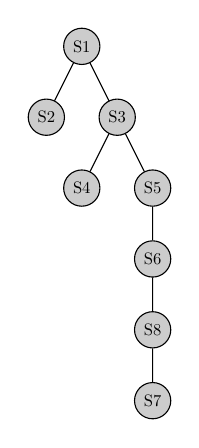
\begin{tikzpicture}[darkstyle/.style={circle,draw,fill=gray!40,minimum size=5,transform shape},scale=0.6]
\node[darkstyle]{S1}
	child{node[darkstyle]{S2}}
    child{node[darkstyle]{S3}
    	child{node[darkstyle]{S4}}
        child{node[darkstyle]{S5}
                child{node[darkstyle]{S6}
                child{node[darkstyle]{S8}
                child{node[darkstyle]{S7}}
                }}}};
\end{tikzpicture}
\caption{Maximum spanning tree of $R$}
\label{fig:corrMST}
\end{subfigure}
\end{figure}

%\[
%\begin{bmatrix}
%0&1&1&1&1&0&0&0\\
%1&0&1&1&0&1&0&0\\
%1&1&0&1&1&1&1&0\\
%1&1&1&0&1&1&0&1\\
%1&0&1&1&0&1&1&1\\
%0&1&1&1&1&0&1&1\\
%0&0&1&0&1&1&0&1\\
%0&0&0&1&1&1&1&0\\
%\end{bmatrix}
%\]
%
%\begin{figure}
%\begin{tikzpicture}
%\foreach \y[count=\xi] in {0,2.2}{
% \foreach \x [count=\yi] in {0,2.5,5,7.5}{
% 
% \ifthenelse{\xi=1}
% {
% \pgfmathtruncatemacro{\label}{(\yi-\xi)+\yi}
% }
% {
% \pgfmathtruncatemacro{\label}{\xi*\yi}
%}
% \node[circle,draw=black,fill=white!80!black,minimum size=5] (\label) at (\x,\y)  {\label} ;
% 
% 
%
%
%}
%}
%\draw (1)--(2) (1)--(3) (1)--(4) (2)--(3) (2)--(4) (3)--(4) (3)--(5) (5)--(7) (7)--(8)
%(6)--(8) (4)--(6) (6)--(5) (4)--(5) (6)--(3) (5)--(8) (6)--(7); 
%
%\draw (1)to[out=0-20,in=200](5);
%\draw (2)to[out=20,in=160](6);
%\draw (3)to[out=0-20,in=200](7);
%\draw (4)to[out=20,in=160](8);
%
%\end{tikzpicture}
%\centering
%\caption{Adjacency graph for the grid.}	
%\label{fig:adjGraph}
%\end{figure}



















